\documentclass[11pt]{article}

\usepackage[a4paper,margin=25mm]{geometry}
\usepackage[T1]{fontenc}
\usepackage[utf8]{inputenc}
\usepackage{lmodern}
\usepackage{microtype}
\usepackage{amsmath,amssymb,amsthm,mathtools}
\usepackage{booktabs}
\usepackage{graphicx}
\usepackage{placeins}
\usepackage{xcolor}
\usepackage{hyperref}
\usepackage[nameinlink,noabbrev]{cleveref}

\hypersetup{
  colorlinks=true,
  linkcolor=blue!55!black,
  citecolor=blue!55!black,
  urlcolor=blue!55!black,
  pdftitle={Exact finite-depth crossings in a Sierpinski--Hanoi free-fermion spin model},
  pdfauthor={Xiaojian Zeng}
}

\newtheorem{theorem}{Theorem}
\newtheorem{lemma}[theorem]{Lemma}
\newtheorem{proposition}[theorem]{Proposition}
\theoremstyle{remark}
\newtheorem{remark}[theorem]{Remark}
\crefname{lemma}{lemma}{lemmas}
\Crefname{lemma}{Lemma}{Lemmas}
\crefname{proposition}{proposition}{propositions}
\Crefname{proposition}{Proposition}{Propositions}

\newcommand{\ii}{\mathrm{i}}
\newcommand{\ones}{\boldsymbol{1}}
\newcommand{\Acal}{\mathcal{A}}
\newcommand{\Z}{\mathbb{Z}}
\newcommand{\R}{\mathbb{R}}

\title{Exact finite-depth crossings in a Sierpinski--Hanoi\\
free-fermion spin model}
\author{Xiaojian Zeng\\
\small PBC School of Finance, Tsinghua University, Beijing 100190, China\\
\small \href{mailto:xiaojianzeng@foxmail.com}{xiaojianzeng@foxmail.com}}
\date{}

\begin{document}
\maketitle

\begin{abstract}
Chapman and Flammia introduced a three-body spin model on a finite
Sierpinski sieve whose fixed symmetry sectors map to free Majorana fermions.
At recursion depth five, their single-particle spectrum contains two marked
levels that were degenerate to numerical precision, and their locations were
conjectured to approach zero with depth.  We resolve this finite-size question
in the sector where every canonical cycle symmetry is $+1$.  A signed
three-copy Schur reduction gives a division-free recurrence for three scalar
polynomials and an exact quotient for the complete characteristic polynomial.
On its flat-band locus, the recurrence can be solved at arbitrary depth.  For
every $k\geq3$ there is a unique nonzero pair of transverse crossings
\[
 J_k^\pm=\pm3^{-(k-3)/2},\qquad
 \lambda_k=\frac12 3^{-(k-3)/2},
\]
where $\lambda$ uses the normalization of the source spectrum.  Each
eigenvalue sign has multiplicity $(3^{k-2}+1)/2$ at the crossing, and
$|J_{k+1}/J_k|=1/\sqrt3$ exactly.  Thus the two depth-five landmarks occur at
$J=\pm1/3$ and $\lambda=1/6$ and are exact crossings rather than avoided
crossings.  We also separate windows that follow the crossing from the fixed
intervals $[1/4,1/2]$ and its negative: on those fixed intervals the tracked
minimum is zero only at $k=5$, with a constructive positive bound otherwise.
All statements concern a finite open, single-particle, all-cycle-$+1$ sector;
they do not establish a many-body gap or a thermodynamic phase transition.
\end{abstract}

\section{Introduction}

Mappings from interacting Pauli Hamiltonians to free fermions turn an
exponentially large spin problem into a single-particle spectral problem.
The frustration-graph framework of Chapman and Flammia characterizes an
important class of such mappings in terms of line graphs and their root
graphs~\cite{ChapmanFlammia2020}.  Related graph-based constructions extend
the class of hidden free-fermion models and connect their spectral properties
to graph invariants~\cite{ElmanChapmanFlammia2021,ChapmanFlammiaKollar2022}.

The final example of Ref.~\cite{ChapmanFlammia2020} is a three-body $XYZ$
model on a recursively constructed Sierpinski sieve.  In a fixed cycle sector
its frustration graph is a Hanoi graph and its root graph supports a free
Majorana hopping problem.  A local Pauli field attaches pendant Majorana modes
to the root graph.  At depth $k=5$, two circled features in the numerical
single-particle spectrum become degenerate within the reported precision.
Their locations move toward $J=0$ as the depth grows, suggesting a finite-size
trace of the scale symmetry of the infinite fractal.  The source does not
determine whether the finite-size meetings are exact, nor does it give their
locations or an all-depth characteristic recurrence.

Self-similar recurrences also occur in other statistical models on Sierpinski
and Hanoi lattices~\cite{Alvarez2023}, but those recurrences do not include the
cycle-sector signs, local-field pendants, or Majorana observable considered
here.  A bounded search of the defining work and the related primary works
above found no earlier expression for the signed recurrence or the crossing
law derived below.  This is necessarily a bounded literature statement, not
an exhaustive priority claim.

\paragraph{Contributions.}
The assumptions and results are as follows.
\begin{enumerate}
  \item We fix the finite open geometry, the canonical all-cycle-$+1$ sector,
  and the source normalization before taking a Schur complement.
  \item We prove that the signed three-copy composition has a depth-independent
  gauge representative.  Its three-corner response closes on two rational
  scalars, which admit a cancellation-safe polynomial lift $(A_k,U_k,D_k)$.
  \item We solve this recurrence exactly on the cycle-flat locus and obtain the
  complete residual factor.  This proves the location, multiplicity, channel,
  transversality, and $1/\sqrt3$ scale ratio of the unique nonzero crossing.
  \item We distinguish a moving continuation window from the fixed intervals
  used to define an avoided-crossing question, and derive a positive
  coefficient-norm bound whenever the exact crossing is outside the latter.
\end{enumerate}
No minimality claim is made for the three-scalar state, and no no-go statement
is made about every possible relation involving characteristic polynomials
alone.

\section{Model, sector, and normalization}
\label{sec:model}

Let $k\geq1$ denote the recursion depth, with $k=1$ a single upright
three-qubit cell.  For each ordered cell $(i,j,\ell)$, the Pauli labels are
$X,Y,Z$ at the lower-left, lower-right, and top vertices, respectively.  In
units where the three-body coupling is one, the finite open Hamiltonian is
\begin{equation}
 H_k(J)=\sum_{(i,j,\ell)\in\mathcal N_k}X_iY_jZ_\ell
       +J\sum_{q\in B_k}\sigma_q^{a_q},\qquad J\in\R.
 \label{eq:spin-hamiltonian}
\end{equation}
Here $B_k$ contains the qubits shared by two cells, and $a_q$ is the third
Pauli label not used at $q$ by those cells.  This is precisely the local-field
augmentation of Eqs.~(72) and (77) of Ref.~\cite{ChapmanFlammia2020}.

At $J=0$, the frustration graph is the three-peg Hanoi graph $H_3^{k-1}$.
The root graph has
\begin{equation}
 |V(R_k)|=\frac{5\,3^{k-2}+3}{2}\quad(k>1),\qquad
 c_k=\frac{3^{k-2}-1}{2}\quad(k>2)
 \label{eq:counts}
\end{equation}
vertices and independent cycles, respectively.  The local field appends one
dedicated Majorana mode to every degree-two root vertex, excluding the three
corners.  We select the sector in which the canonical Hermitian generator of
every fundamental cycle has eigenvalue $+1$.  This selection fixes the cycle
products of the oriented hopping graph; changes of spanning tree or edge
orientation are thereafter only diagonal Majorana gauges.

Write the free-fermion Hamiltonian in the convention of the source as
\begin{equation}
 \widetilde H_k=\ii\gamma h_k(J)\gamma^{\mathsf T}
 =2\ii\sum_{a<b}h_{k,ab}(J)\gamma_a\gamma_b.
 \label{eq:source-h}
\end{equation}
A Pauli term with coefficient $w\in\{1,J\}$ therefore produces an oriented
entry $h_{ab}=\pm w/2$.  It is convenient to remove this factor by defining
the real antisymmetric matrix
\begin{equation}
 \Acal_k(J)=2h_k(J),\qquad
 C_k(z,J)=\det\!\left(zI-\Acal_k(J)\right).
 \label{eq:char-def}
\end{equation}
The physical Hermitian matrix is $\ii\Acal_k$.  If $x$ is one of its positive
eigenvalues, the ordinate in the source figure is $\lambda=x/2$.  This
single-particle quantity is not a many-body excitation gap; a physical parity
projection would be required for that interpretation.

\section{Signed self-similarity and the Schur state}
\label{sec:schur}

We first isolate the sign information that survives recursive composition.

\begin{lemma}[Depth-independent signed composition]
\label{lem:sign}
For every $k\geq2$, the depth-$(k+1)$ augmented root graph consists of three
prefix copies of the depth-$k$ graph, joined at three pairwise-distinct
interface vertices that acquire three new pendants.  In the all-cycle-$+1$
sector, each copy is vertex-gauge equivalent to $\Acal_k$, and the quotient
macrocycle has one fixed gauge orbit.  In a representative of that orbit, the
three effective interface signs are $(+,+,-)$.
\end{lemma}

\begin{proof}
Prefixing the Hanoi address by $0,1,$ or $2$ translates an upright cell but
preserves its ordered $X,Y,Z$ labels.  Hence every internal cycle product of a
prefix copy equals the corresponding depth-$k$ product.  Equality of all cycle
products is exactly the vertex-gauge criterion for signed graphs, so each
restriction is gauge equivalent to $\Acal_k$.

The cycle ranks satisfy $c_{k+1}=3c_k+1$, leaving one quotient cycle after the
three copy cycle spaces are removed.  Its cross-copy term pairs are
\begin{equation}
 (01\cdots1,10\cdots0):Y/X,\quad
 (02\cdots2,20\cdots0):Z/X,\quad
 (12\cdots2,21\cdots1):Z/Y.
 \label{eq:cross-copy}
\end{equation}
Within a prefix copy, the two interface ports have a unique side geodesic.
Its length obeys $L_2=2$ and $L_{k+1}=2L_k$, hence
$L_k=2^{k-1}$.  Multiplying the translated Pauli terms along the three side
paths cancels internal factors pairwise.  The Hermitianizing phase is
$-3L_k$ modulo four, whereas the unsigned Majorana loop contributes $3L_k$
modulo four.  The cycle-orientation rule of Ref.~\cite{ChapmanFlammia2020}
therefore fixes the oriented quotient product to $+1$ in the selected sector.

In the large-$z$ Schur expansion of $zI-\Acal$, an off-diagonal port response
starts with minus the oriented product along its unique shortest path.  The
product of the three effective copy couplings is consequently
$(-1)^3(+1)=-1$.  Six independent port gauges reduce every compatible signing
to a representative with interface signs $(+,+,-)$, proving the claim.
\end{proof}

After eliminating all vertices except the three outer corners, permutation
symmetry and a fixed boundary gauge put the corner Schur complement in the
form
\begin{equation}
 S_k=\alpha_k I_3+\beta_k(\ones\ones^{\mathsf T}-I_3).
 \label{eq:corner-response}
\end{equation}
Let $\delta_k^{\rm int}$ be the determinant of the eliminated interior block.  After adding
the two copy contributions at each interface, correcting the duplicated
diagonal $z$, and eliminating the new pendant, define
\begin{equation}
 q_k=2\alpha_k-z+\frac{J^2}{z}.
 \label{eq:q-def}
\end{equation}
In the representative of Lemma~\ref{lem:sign}, the interface and coupling blocks
are
\begin{equation}
 \mathcal C_k=
 \begin{pmatrix}
 q_k&\beta_k&\beta_k\\
 \beta_k&q_k&-\beta_k\\
 \beta_k&-\beta_k&q_k
 \end{pmatrix},\qquad
 \mathcal B_k=
 \begin{pmatrix}
 \beta_k&\beta_k&0\\
 \beta_k&0&\beta_k\\
 0&\beta_k&-\beta_k
 \end{pmatrix}.
 \label{eq:interface-blocks}
\end{equation}
Direct $3\times3$ elimination gives
\begin{equation}
 \det\mathcal C_k=(q_k-2\beta_k)(q_k+\beta_k)^2
 \label{eq:interface-det}
\end{equation}
and, after the output gauge $\operatorname{diag}(1,-1,-1)$,
\begin{subequations}
\label{eq:rational-update}
\begin{align}
 \alpha_{k+1}&=\alpha_k-\frac{2\beta_k^2}{q_k+\beta_k},\\
 \beta_{k+1}&=\frac{\beta_k^2}{q_k+\beta_k},\\
 \delta_{k+1}^{\rm int}&=(\delta_k^{\rm int})^3z^3
 (q_k-2\beta_k)(q_k+\beta_k)^2.
\end{align}
\end{subequations}
The rational form is compact, but it can hide characteristic factors when a
corner response has a pole.  The following polynomial lift retains them.

\begin{theorem}[Division-free characteristic recurrence]
\label{thm:recurrence}
Define scalar polynomials $A_k,U_k,D_k\in\Z[J,z]$ at depth two by
\begin{equation}
 A_2=z^2+1,\qquad U_2=1,\qquad D_2=z.
 \label{eq:base}
\end{equation}
For every $k\geq2$, set
\begin{subequations}
\label{eq:polynomial-update}
\begin{align}
 r_k&=2A_k+1+(J^2-z^2)U_k,\\
 A_{k+1}&=A_kr_k-2,\\
 U_{k+1}&=U_kr_k,\\
 D_{k+1}&=D_k^3U_k(r_k-3).
\end{align}
\end{subequations}
Then the complete characteristic polynomial of \cref{eq:char-def} is
\begin{equation}
 \boxed{C_k(z,J)=
 \frac{D_k(A_k+2)(A_k-1)^2}{z^3U_k}.}
 \label{eq:char-quotient}
\end{equation}
The quotient is exact in $\Z[J,z]$.
\end{theorem}

\begin{proof}
Substitute
\begin{equation}
 \alpha_k=\frac{A_k}{zU_k},\qquad
 \beta_k=\frac{1}{zU_k},\qquad \delta_k^{\rm int}=D_kU_k^2
 \label{eq:poly-substitution}
\end{equation}
into \cref{eq:q-def,eq:rational-update}.  Clearing the common denominators
gives \cref{eq:polynomial-update}; adjoining the three corners gives
\cref{eq:char-quotient}.  The derivation is initially an identity in
$\mathbb Q(J,z)$, where the Schur inverses exist.  Multiplication by the
displayed denominators gives a polynomial identity, so it extends to their
zero loci.  The depth-two matrix verifies \cref{eq:base}.  Induction then
places $A_k,U_k,D_k$ in $\Z[J,z]$ and proves exact divisibility at each depth.
In particular, flat factors cancelled from the rational corner response
remain in $D_k$.
\end{proof}

\section{Solution on the flat locus}
\label{sec:flat}

Put
\begin{equation}
 t=J^2,\qquad y=z^2,\qquad s=t+y.
 \label{eq:flat-vars}
\end{equation}
Under $z=-\ii x$, the locus $s=0$ is the physical flat band $x=|J|$.

\begin{lemma}[Restricted recurrence]
\label{lem:restricted}
For every $k\geq2$, restriction to $s=0$ gives
\begin{equation}
 A_k=1-3^{k-2}t,\qquad U_k=3^{k-2},\qquad r_k=3.
 \label{eq:restricted-solutions}
\end{equation}
Moreover $r_k-3=sR_k(s,t)$ exactly, with
\begin{equation}
 R_k(0,t)=5^{k-2}.
 \label{eq:R-value}
\end{equation}
\end{lemma}

\begin{proof}
The base case follows from \cref{eq:base}.  On $s=0$ one has $z^2=-t$ and
$J^2-z^2=2t$.  If the first two identities in
\cref{eq:restricted-solutions} hold, their $t$ contributions cancel in
$r_k$, leaving $r_k=3$; the $A$ and $U$ updates then prove the next depth.

For the transverse quotient, differentiate at fixed $t$ with respect to $s$
and restrict to $s=0$.  A dot denotes this operation and
$T_k=R_k(0,t)$.  Since $J^2-z^2=2t-s$,
\begin{equation}
 T_k=2\dot A_k-U_k+2t\dot U_k.
 \label{eq:T-def}
\end{equation}
Differentiating the two updates gives
\begin{equation}
 \dot A_{k+1}=3\dot A_k+A_kT_k,\qquad
 \dot U_{k+1}=3\dot U_k+U_kT_k.
 \label{eq:dot-update}
\end{equation}
On the locus, $A_k+tU_k=1$, so substitution into \cref{eq:T-def} yields
$T_{k+1}=5T_k$.  Since $T_2=1$, \cref{eq:R-value} follows.
\end{proof}

The factor retained by $D_k$ can now be counted without a genericity
assumption.

\begin{proposition}[Complete residual factor]
\label{prop:residual}
Let $c_k=(3^{k-2}-1)/2$.  Then $s^{c_k}$ divides $D_k$ exactly.  If
$\overline D_k=D_k/s^{c_k}$, then on $s=0$
\begin{equation}
 \overline D_k=b_kz^{3^{k-2}},\qquad
 b_k=15^{(3^{k-2}-2k+3)/4}>0.
 \label{eq:Dbar}
\end{equation}
Consequently, for $t>0$,
\begin{equation}
 \left.\frac{C_k}{s^{c_k}}\right|_{s=0}
 =(-1)^{c_k-1}b_k3^{k-1}t^{c_k+1}
   \left(1-3^{k-3}t\right).
 \label{eq:complete-residual}
\end{equation}
\end{proposition}

\begin{proof}
The $D$ update in \cref{eq:polynomial-update} and
Lemma~\ref{lem:restricted} show that the flat exponent obeys
$c_{k+1}=3c_k+1$ with $c_2=0$, giving the stated $c_k$.  The quotient is
nonzero because $R_k(0,t)=5^{k-2}$.  The remaining coefficient obeys
$b_2=1$ and $b_{k+1}=b_k^3 15^{k-2}$, whose solution is
\cref{eq:Dbar}.  Finally insert \cref{eq:restricted-solutions,eq:Dbar} into
\cref{eq:char-quotient}.  All factors are nonzero for $t>0$ except the one
shown explicitly, proving both completeness and \cref{eq:complete-residual}.
\end{proof}

\section{Exact crossings and scale law}
\label{sec:crossings}

\begin{theorem}[Finite-depth crossing sequence]
\label{thm:crossing}
In the finite open all-cycle-$+1$ single-particle sector, every integer
$k\geq3$ has exactly one nonzero positive collision on the cycle-flat locus,
together with its $J\mapsto-J$ gauge twin:
\begin{equation}
 \boxed{
 J_k^\pm=\pm3^{-(k-3)/2},\quad
 x_k=3^{-(k-3)/2},\quad
 \lambda_k=\frac12 3^{-(k-3)/2}.}
 \label{eq:crossing-sequence}
\end{equation}
For either physical eigenvalue sign $\pm x_k$, the generic flat multiplicity
$c_k$ increases to $c_k+1=(3^{k-2}+1)/2$.  The additional branch is the
boundary-symmetric channel.  The crossing is transverse at every finite
depth and
\begin{equation}
 \frac{|J_{k+1}|}{|J_k|}
 =\frac{\lambda_{k+1}}{\lambda_k}=\frac{1}{\sqrt3}.
 \label{eq:scale-ratio}
\end{equation}
\end{theorem}

\begin{proof}
By Proposition~\ref{prop:residual}, a nonzero collision requires and is implied by
$1-3^{k-3}t=0$.  This has the unique positive solution
$t=3^{-(k-3)}$, proving the locations and \cref{eq:scale-ratio}.  The exact
pendant gauge $\Acal_k(-J)=G\Acal_k(J)G$ for a diagonal sign matrix $G$
supplies the negative twin.

The factor $s^{c_k}$ gives $c_k$ flat modes for each eigenvalue sign.  The
remaining factor in \cref{eq:complete-residual} has a simple root, so the
multiplicity becomes $c_k+1$.  Since $\ii\Acal_k$ is Hermitian, algebraic and
geometric multiplicities coincide.

To identify the extra branch, the boundary-symmetric eigenvalue of
\cref{eq:corner-response} satisfies the recurrence identity
\begin{equation}
 \alpha_k+2\beta_k
 =\frac{A_k+2}{zU_k}
 =\frac{A_{k-1}}{zU_{k-1}}.
 \label{eq:symmetric-channel}
\end{equation}
Its flat-locus zero is exactly the last factor of
\cref{eq:complete-residual}.  The two orthogonal corner channels carry
$A_k-1$, which does not vanish there; the persistent cycle-flat modes have
zero corner response.

For transversality, set $n=k-3$.  Differentiating the recurrence at the
collision gives
\begin{equation}
 \partial_y A_{k-1}
 =\frac{5^{n+1}+6\,3^n+1}{12}>0.
 \label{eq:partial-y}
\end{equation}
Implicit differentiation of $A_{k-1}(J^2,-x^2)=0$ then yields
\begin{equation}
 \left.\frac{dx_{\mathrm{disp}}}{dJ}\right|_{J_k^+}
 =\frac{5^{n+1}-6\,3^n+1}{5^{n+1}+6\,3^n+1}.
 \label{eq:disp-slope}
\end{equation}
The flat branch has slope one, and their leading separation in $x$ is
\begin{equation}
 \frac{12\,3^n}{5^{n+1}+6\,3^n+1}|J-J_k^+|,
 \label{eq:linear-separation}
\end{equation}
which is strictly positive for every finite $n$.
\end{proof}

The first depths are summarized in \cref{tab:sequence}.  The depth-five
entry establishes that the marked source features occur at $J=\pm1/3$ and
$\lambda=1/6$, with multiplicity fourteen per eigenvalue sign.  The exact
sequence and its transverse coefficients are shown in \cref{fig:scale}.

\begin{table}[!htbp]
\centering
\caption{First members of the exact crossing sequence.  Multiplicity is for
one eigenvalue sign.  The last column is the dispersive slope in
\cref{eq:disp-slope}; the flat-band slope is one.}
\label{tab:sequence}
\begin{tabular}{ccccc}
\toprule
$k$ & $|J_k|$ & $\lambda_k$ & multiplicity & $dx_{\rm disp}/dJ$\\
\midrule
3 & $1$ & $1/2$ & $2$ & $0$\\
4 & $1/\sqrt3$ & $1/(2\sqrt3)$ & $5$ & $2/11$\\
5 & $1/3$ & $1/6$ & $14$ & $2/5$\\
6 & $1/(3\sqrt3)$ & $1/(6\sqrt3)$ & $41$ & $116/197$\\
7 & $1/9$ & $1/18$ & $122$ & $220/301$\\
\bottomrule
\end{tabular}
\end{table}

\begin{figure}[!htbp]
\centering
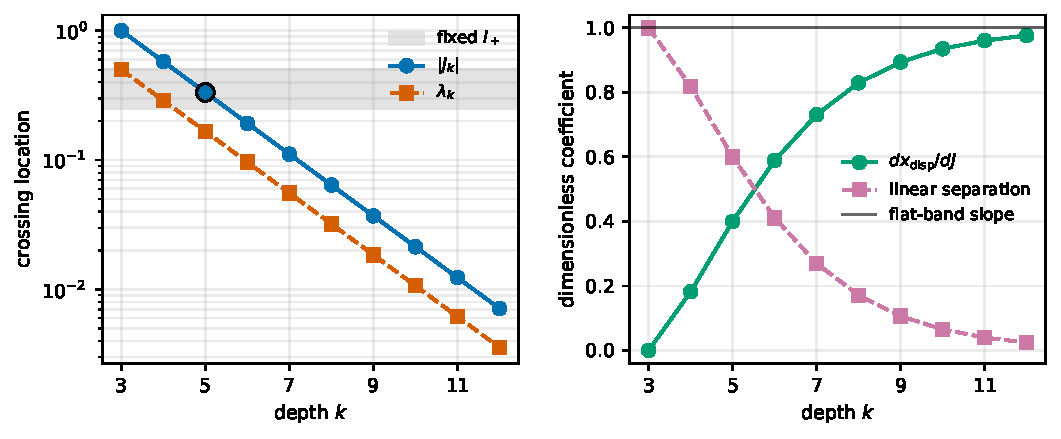
\includegraphics[width=\textwidth]{figures/crossing_scale.pdf}
\caption{Closed-form finite-depth predictions, with no fitted parameters.
Left: the crossing locations $|J_k|$ and source ordinates $\lambda_k$; the
gray strip is $I_+=[1/4,1/2]$, and the open circle marks the depth-five source
landmark.  Right: the dispersive slope and the coefficient of the linear
separation in $x$.  The two branches remain transverse at every finite depth,
although their slope difference tends to zero.}
\label{fig:scale}
\end{figure}
\FloatBarrier

\section{Fixed intervals versus moving windows}
\label{sec:windows}

An all-depth crossing sequence does not imply zero minimum gap on a fixed
parameter interval after the crossing leaves it.  For the positive side,
define $I_+=[1/4,1/2]$ and let $\Delta_k^+$ be the minimum source-$\lambda$
separation between the tracked flat and boundary-symmetric branches on
$I_+$.  Let $I_-=-I_+$ and define $\Delta_k^-$ by the gauge-related negative
branches.

Set
\begin{equation}
 F_k(x,J)=A_{k-1}(z=-\ii x,J)=\sum_{p,q}c_{pq}J^px^q,
 \label{eq:F-def}
\end{equation}
and the explicit coefficient norm
\begin{equation}
 M_k=\sum_{\substack{p\geq0\\q\geq1}}
 q|c_{pq}|\,2^p4^{q-1}.
 \label{eq:M-def}
\end{equation}
Every relevant eigenvalue obeys $|x|\leq4$ for $|J|\leq2$ by the row-sum
bound, and therefore $|\partial_xF_k|\leq M_k$ in this box.  On the flat
branch,
\begin{equation}
 F_k(J,J)=1-3^{k-3}J^2.
 \label{eq:F-flat}
\end{equation}
Its minimum absolute value on $I_+$ is
\begin{equation}
 d_k=
 \begin{cases}
 3/4,&k=3,\\
 1/4,&k=4,\\
 0,&k=5,\\
 3^{k-3}/16-1,&k\geq6.
 \end{cases}
 \label{eq:d-values}
\end{equation}
For $k\neq5$, the mean-value theorem between $x=J$ and any zero of the
tracked dispersive factor gives
\begin{equation}
 \boxed{\Delta_k^\pm\geq\frac{d_k}{2M_k}>0.}
 \label{eq:fixed-gap-bound}
\end{equation}
The factor $1/2$ converts $x$ to the source ordinate $\lambda$.  At $k=5$,
$J_5=1/3\in I_+$ and \cref{thm:crossing} gives
$\Delta_5^\pm=0$.  Hence the fixed-interval minimum is zero if and only if
$k=5$.

By contrast, the moving windows
\begin{equation}
 W_k^+=[J_k/2,3J_k/2],\qquad W_k^-=-W_k^+
 \label{eq:moving-windows}
\end{equation}
contain the exact crossing for every $k\geq3$, so their minima are always
zero.  This distinction prevents a moving finite-size landmark from being
misreported as an avoided crossing on a fixed experimental control range.

\section{Exact and independent checks}
\label{sec:checks}

The model input was reconstructed in two representations: directly from the
oriented Pauli cells and independently from legal Hanoi moves followed by a
Krausz-root construction.  At $k=5$ both representations give 81 root edges,
69 root vertices, 39 pendant modes, and a 108-dimensional antisymmetric
matrix.  Every cycle product is $+1$ in the selected convention.  Across the
full plotted range $J\in[-2,2]$, all 18 raster-resolvable branches of the
source figure agree with the reconstructed spectrum within the resolution of
the raster.

An exact $\Z[J,x]$ factorization at $k=5$ contains
\begin{equation}
 x^{24}(J^2-x^2)^{13}(J^2-x^2+3)^3
 (J^2-x^2+5)^4G_8(x,J),
 \label{eq:k5-selected-factors}
\end{equation}
times factors that are nonzero at the target.  The relevant degree-eight
factor is
\begin{align}
 G_8={}&x^8-9x^6+24x^4-17x^2+1\notag\\
 &+J^2(-3x^6+19x^4-30x^2+8)\notag\\
 &+J^4(3x^4-11x^2+6)+J^6(1-x^2).
 \label{eq:G8}
\end{align}
On $x=|J|$, $G_8=1-9J^2$.  At $J=x=1/3$ one has
$\partial_JG_8=4$ and $\partial_xG_8=-10$, recovering the slope $2/5$ and
showing directly that the depth-five meeting is transverse.

The recurrence was then frozen before direct higher-depth comparisons.  At
$k=6$, a separately constructed 324-mode matrix has 40 cycle-flat modes per
eigenvalue sign.  At $J=1/(3\sqrt3)$, exact arithmetic in two finite fields
and both square-root embeddings gives flat-factor multiplicity 41 and rank
242 for $\Acal_6^2+J^2I$.  Real Hermitian diagonalization finds 41 positive
target eigenvalues, a separation exceeding $0.0275$ from the nearest unrelated
level, and the predicted order exchange.  A further independent $k=7$
reconstruction gives 122 positive target modes at $J=x=1/9$, with the closest
unrelated level separated by $0.00988$ and the centered slope agreeing with
$220/301$.  These finite calculations are adversarial checks; the arbitrary-
depth statement rests on the signed-copy and polynomial inductions above.

The accompanying reproducibility package contains the exact symbolic
producers, independently structured checkers, serialized graph inputs, and
the short script generating \cref{fig:scale}.  The accepted computations used
Python 3.12.14, NumPy 2.3.5, SciPy 1.18.1, SymPy 1.14.0, and python-flint
0.9.0.  Floating-point results are not used as certificates of the exact
identities.

\section{Physical interpretation and limitations}
\label{sec:discussion}

The recurrence reduces the characteristic calculation for an exponentially
growing signed graph to three scalar polynomial updates.  More importantly,
it retains the cycle-flat factors that disappear from a naive rational corner
response.  The source's two numerical landmarks are therefore an exact
finite-depth, scale-covariant sequence: their locations shrink geometrically,
while each finite-depth meeting remains a transverse Hermitian crossing.
The boundary-symmetric channel identity in \cref{eq:symmetric-channel}
specifies which dispersive state joins the growing cycle-flat space.

The result is deliberately narrower than a statement about the full spin
spectrum.  It applies only to the finite open geometry and the canonical
all-cycle-$+1$ sector.  Other cycle sectors have different signed holonomies.
No physical fermion-parity projection has been imposed, so $\lambda_k$ is not
asserted to be a many-body gap.  The limit $J_k\to0$ and the exact ratio
$1/\sqrt3$ show finite-size scale covariance of this collision sequence, but
do not prove a phase transition, critical field theory, experimental
realization, or universal behavior of other fractal models.  Finally, the
three-scalar recurrence is constructive; its minimality among all possible
recurrences has not been established.

\section*{Data and code availability}

The LaTeX source, exact-certificate scripts, checker scripts, serialized graph
inputs, and figure-generation code accompany this draft.  A stable public
archive and license statement must be selected by the author before
submission; no external repository or journal submission is claimed here.

\section*{Author contributions and use of computational tools}

Xiaojian Zeng is the prospective author of this draft; the final contribution
statement and responsibility for the work remain subject to his confirmation.
A large language model was used extensively in problem development,
literature screening, derivations, symbolic and numerical calculations, code
and figure production, independent computational checks, and manuscript
drafting.  The prospective author has not yet certified those outputs.  Before
submission, he must independently review the primary sources, proofs, code,
numerical evidence, bibliography, disclosure, and institutional details and
must make any corrections needed to assume full responsibility for the work.

\section*{Acknowledgments}

No funding statement has been supplied for this draft.  The author should add
an accurate statement before submission.

\bibliographystyle{unsrturl}
\bibliography{references}

\end{document}
